%versi 3 (22-07-2020)
\chapter{Landasan Teori}
\label{chap:teori}
Pejelasan tentang teori-teori yang perlu diketahui sebelum pembuatan laman web. 

\section{\textit{Command-line Interface}}
\label{sec:CLI}
%jangan lupa tambahakan cite
\textit{Command-line interface}(CLI) merupakan sebuah antarmuka pengguna yang berbasis teks yang digunakan untuk menjalankan program, mengelola berkas-berkas pada komputer, dan dapat berinteraksi dengan komputer.\textit{Command-line interface} juga disebut sebagai \textit{command-line user interfaces}, \textit{console user interfaces}, dan \textit{character user interfaces}. \textit{Command-line interface} menerima sebuah perintah yang diinput melalui keyboard perintah yang dipanggil oleh \textit{command prompt} yang dijalankan oleh komputer.

\textit{Command-line interface} lansung dapat berfungsi ketika sistem komputer dijalakan. \textit{Command-line interface} dapat terbuka di layar kosong dengan \textit{command prompt} lalu perintah-perintah dapat dimasukkan.   
 
\begin{figure}[H]
	\centering
	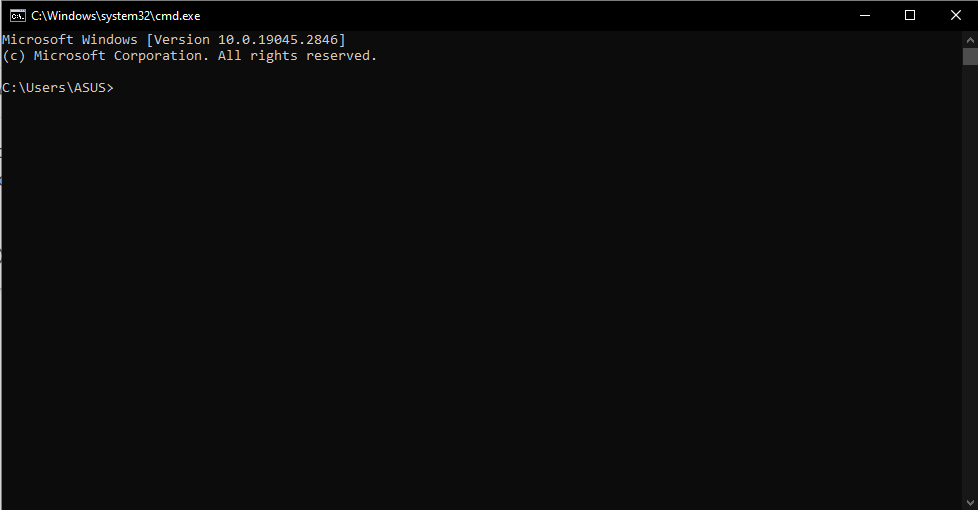
\includegraphics[width=0.8\textwidth]{Gambar/commandprompt.png}
	\caption{\textit{Command Prompt}}
	\label{fig:cmd}
\end{figure}

Jenis perintah-perintah dari \textit{Command-line interface} akan berisikan :

\begin{enumerate}
	\item Perintah-perintah dari sistem yang dikodekan sebagai bagian dari antarmuka sistem operasi
	\item Program yang dapat dijalankan ketika berhasil dipanggil,dan menjalakan aplikasi yang berbasis teks atau grafis.
	%tambahkan footnote untuk batch program
	\item \textit{batch program}(\textit{batch files} atau \textit{shell script}) yang merupakan berkas teks berisikan urutan perintah-perintah. Ketika perintah berhasil dipanggil, \textit{batch program} akan menjalakan perintahnya yang mungkin berisikan sebuah perintah sistem dan program yang dapat dieksekusi.
\end{enumerate}
%tambahakan cite untuk scp referensi buku
Perintah \textit{Command-line interface} yang digunakan antaralain :
\subsection{SCP(\textit{Secure Copy Protocol})}
Salah satu perintah yang terdapat pada \textit{Command-line interface} yaitu SCP(\textit{secure copy}). SCP memiliki fungsi yang mirip seperti pada perintah \emph{cp}(\textit{copy}) yaitu untuk meyalin berkas. Perbedaannya yang paling terlihat terletak pada sumber atau tujuan ke \textit{remote host}. Sebagai contoh, jika ingin menyalin sebuah dokumen dari \textit{home directory}(berkas dalam komputer) ke \textit{remote system}, atau dari \textit{working directory} ke sistem lokal. 

\begin{figure}[H]
	\centering
	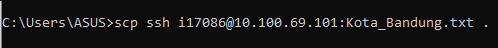
\includegraphics[width=0.8\textwidth]{Gambar/scp.png}
	\caption{Pemanggilan SCP}
	\label{fig:scp}
\end{figure}

Gambar \ref{fig:scp} merupakan contoh penyalinan berkas Kota\textunderscore Bandung.txt. Berkas tersebut yang tersimpan didalam \textit{remote host} dan disalin ke \textit{local system} pengguna.


\section{Hadoop Distributed File System}
\label{sec:hdfs}
%HDFS \textit{Hadoop Distributed File System} merupakan sistem file yang terdistribusi yang dapat diakses oleh pengguna untuk membaca(\textit{read}) dan menulis(\textit{write}) data. HDFS digunakan untuk sebagai tempat penyimpanan berkas-berkas yang berukuran besar pada \textit{Hadoop}.
HDFS (\textit{Hadoop Distributed File System}) merupakan sistem file terdisribusi yang berada pada penyimpanan server dan memiliki banyak kesamaan pada \textit{base storage system}. Sistem penyimpanan terdistribusi ini dapat menyimpan data dalam jumlah yang sangat besar melalui jaringan komputer dengan redudansi bawaan untuk melindungi data. HDFS dirancang untuk pemrosesan yang cepat dan toleran terhadap kesalahan, sehingga memungkinkan pengguna \textit{hardware} pada penyimanan tidak terkana biaya yang mahal.

HDFS memungkinkan para pengguna untuk menyimpan data kedalam file yang dibagi menjadi beberapa \textit{block}. Karena \textit{Hadoop} dirancang untuk bekerja dengan jumlah data yang besar, ukuran \textit{block} pada HDFS jauh lebih besar daripada yang digunakan oleh \textit{typical relational databases}. Dengan ukuran awal \textit{block} sebesar 128MB, dan dapat dikonfigurasi ukurannya mencapai 512MB.
%cite buku Sam R.Alapati

HDFS memiliki 2 jenis \textit{node}, yaitu \textit{namenode} sebagai \textit{node master} dan \textit{datanode} sebagai \textit{node slave}. Kelebihan utama yang ditawarkan HDFS adalah \textit{scalability} dan \textit{availability} yang dicapai dikarenakan memiliki kemampuan replikasi data dan \textit{fault tolerance}.Dengan adanya kemampuan replikasi data/file, ketika ada kegagalan \textit{software }atau \textit{hardware}, HDFS akan melakukan replikasi ulang blok-blok data pada \textit{node} yang mengalami kegagalan.
%cite buku hadoop in practice

Semua perintah HDFS dipanggil menggunakan \textit{script} \textit{bin/hdfs}. Penjalanan \textit{script} \textbf{"hdfs"} tanpa argumen akan mencetak deskripsi untuk semua perintah.
\begin{figure}[H]
	\centering
	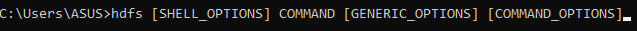
\includegraphics[width=0.8\textwidth]{Gambar/hdfs2.png}
	\caption{Perintah HDFS CLI}
	\label{fig:hdfs}
\end{figure}
Gambar \ref{fig:hdfs} merupakan pemanggilan perintah pada HDFS. Setiap opsi perintah memiliki fungsi untuk menajalankan \textit{script} pada CLI. Penjelasan tiap opsi dijelaskan pada tabel \ref{table:command_options}.  

\begin{table}[h]
	\caption{\label{table:command_options}\textit{Hadoop} memiliki opsi \textit{parsing framework} yang menjelaskan setiap fungsi kelasnya }
	\begin{tabular}{|l|l|}
		\hline
		\textbf{COMMAND\_OPTION} & \textbf{Deskripsi}                                            \\ \hline
		SHELL\_OPTIONS           & kumpulan shell\_option  yang umum                             \\ \hline
		GENERIC\_OPTIONS         & kumpulan generic\_option yang didukung oleh beberapa perintah \\ \hline
		COMMAND COMMAND\_OPTIONS & Bermacam perintah dengan opsi                                 \\ \hline
	\end{tabular}
\end{table}
\newpage

Penggunaan perintah HDFS yang digunakan antara lain :
\begin{enumerate}
	\item Penggunaan perintah \textbf{dfs}\\
	Perintah \textbf{dfs} digunakan untuk menjalankan(\textit{run}) perintah \textit{filesystem} yang didukung oleh \textit{Hadoop}. \textit{\textbf{[COMMAND\_OPTIONS]}} dapat dilihat pada \href{https://hadoop.apache.org/docs/stable/hadoop-project-dist/hadoop-common/FileSystemShell.html}{\textit{File System Guide}}. Contoh pemanggilan \textbf{dfs} seperti pemanggilan pada Gambar \ref{fig:dfs}
	\begin{figure}[H]
		\centering
	%	\captionsetup{width=.9\linewidth}
		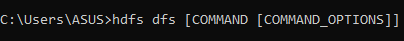
\includegraphics[width=0.8\textwidth]{Gambar/dfs.png}
		\caption{Perintah HDFS dfs}
		\label{fig:dfs}
	\end{figure}
	\item Penggunaan perintah \textbf{get}\\
	Perintah \textbf{get} digunakan untuk menyalin file HDFS ke \textit{local system}.Gambar \ref{fig:get} merupakan contoh yang menunjukkan cara penggunaan perintah \textbf{-get} untuk mengunduh file dari HDFS ke \textit{local file system}
	\begin{figure}[H]
		\centering
	%	\captionsetup{width=.9\linewidth}
		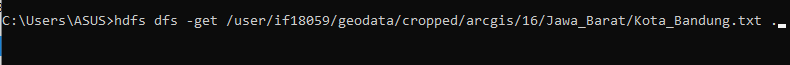
\includegraphics[width=0.8\textwidth]{Gambar/get.png}
		\caption{Perintah HDFS dfs -get untuk mengunduh file HDFS Kota\_Bandung.txt ke \textit{local system}}
		\label{fig:get}
	\end{figure}
	\item Penggunaan perintah \textbf{-ls}\\
	Perintah \textbf{-ls} digunakan untuk menampilkan daftar isi \textit{directory} yang ditentukan oleh \textit{path} yang disediakan oleh pengguna. Gambar merupakan contoh yang menunjukkan cara penggunaan perintah \textbf{-ls} untuk melihat isi file HDFS.
	\begin{figure}[H]
		\centering
	%	\captionsetup{width=0.9\textwidth}
		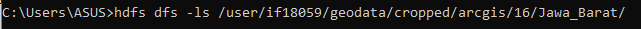
\includegraphics[width=0.8\textwidth]{Gambar/ls.png}
		\caption{Perintah HDFS dfs -ls untuk menampilkan isi file yang berada didalam \textit{directory} Jawa\_Barat}
		\label{fig:ls}
	\end{figure}
\end{enumerate}



\section{\textit{Python}}
\label{sec:python}
%\textit{Python} Merupakan sebuah bahasa pemograman komputer yang dikembangkan khusus untuk membuat \textit{source code} yang mudah untuk dibaca. Bahasa pemograman \textit{pyhton} memiliki \textit{libary} yang lengkap sehingga memudahkan seorang pengembang untuk membuat sebuah aplikasi sesuai dengan keinginan dengan menggunakan \textit{source code} yang terlihat sederhana.
%cite
\textit{Python} adalah bahasa pemrograman yang memulai debutnya pada tahun 1991. \textit{Python} mencakup \textit{object-oriented programming} dan memperkenalkan \textit{syntax} yang membuat banyak \textit{operations} menjadi sangat ringkas dan elegan. Hal yang harus diperhatikan oleh \textit{programmers} baru mengenai \textit{Python} adalah pemakaian spasi(" ") sangat berpengaruh pada arti program yang dikembangkan. Pada proses pengembangan menggunakan bahasa \textit{Python} harus menggunakan \textit{text editor} yang dapat mengenali \textit{syntax}-nya agar memudahkan membuat program sesuai yang diinginkan.
%cite data structures & algorithm in pyhton
Bahasa pemrograman \textit{Python} Merupakan sebuah bahasa pemograman komputer yang dikembangkan khusus untuk membuat \textit{source code} yang mudah untuk dibaca. \textit{Pyhton} memiliki \textit{library} yang lengkap sehingga memudahkan seorang \textit{programmer} untuk membuat sebuah aplikasi sesuai dengan keinginan dengan menggunakan \textit{source code} yang terlihat sederhana.

\subsection{\textit{Pillow (PIL Fork)}}
\label{subsec:python PIL}
\textit{Python Imaging Library} merupakan salah satu \textit{library} yang terdapat pada bahasa pemrograman \textit{Python}.PIL dapat menambahkan pemrosesan gambar ke bahasa pemrograman \textit{Python}.\textit{Library} ini menyediakan \textit{extensive file format}, representasi internal yang efisien, dan memiliki kemampuan yang baik dalam pemrosesan gambar. Pentingnya \textit{library} yang dirancang untuk dapat mengakses data yang disimpan dengan cepat dalam berbagai format piksel. Seharusnya memberikan dasar yang kuat sebagai alat pengolahan gambar
%cite dari website pillow fork doc

\section{\textit{Base64}}
\label{sec:base64}

Base64 merupakan sebuah algoritma yang digunakan untuk mengubah tipe data \textit{bytes} menjadi tipe data yang dapat dilihat(dan sebaliknya). Skema pengkodean biner ke teks pada Base64 sebagai persyaratan untuk mengirim tipe data \textit{bytes} melalui jaringan komunikasi yang tidak mengizinkan tipe data biner tetapi hanya tipe data berbasis teks.Data teks yang dihasilkan terdiri dari berbagai karakter yang terdapat pada standar ASCII. Penggunaan kata Base64 berasal dari jumlah karakter ASCII yang digunakan. 64 karakter yang digunakan antara lain adalah 26 karakter a-z \textit{lowercase}, 26 karakter A-Z \textit{uppercase}, ditambah dengan 2 karakter tambahan yaitu karakter tambah ”+” dan karakter garis miring ”/”. Base64 juga sebenarnya memiliki karakter ke 65 yaitu karakter sama dengan ”=” yang digunakan sebagai \textit{padding}. Karakter sama dengan (”=”) digunakan pada segmen terakhir data biner yang tidak memiliki total 6 \textit{bit}. Keseluruhan karakter yang digunakan pada Base64 disebut juga tabel enkoding Base64.

Base64 bekerja dengan cata memotong data biner menjadi segmen-segmen berukuran 6 \textit{bit}. Base64 hanya menggunakan 6 \textit{bit} untuk bisa memenuhi seluruh karakter yang digunakan (26 = 64). Masing-masing segmen tersebut kemudian dibaca ke dalam tipe desimal lalu dikonversi ke karakter ASCII. Sebagai contoh konversi data yang berisi 3 buah \textit{byte} yaitu 155, 162, dan 233. Tipe data \textit{byte} diubah menjadi data biner dan diambung menjadi satu yaitu 100110111010001011101001. Kemudian data biner dipotong menjadi segmen yang berisi 6 \textit{bit} menjadi 100110, 111010, 001011, 101001. Masing-masing data dikonversi menjadi desimal , 58, 11, 4yaitu 381. Terakhir data dikonversikan ke karakter ASCII yang berada pada tabel enkoding Base64 menjadi m6Lp. Cara yang sama namun terbalik prosesnya digunakan untuk mendeskripsi data dari Base64 kembali ke tipe data \textit{byte}.
%cite skripsi juan

\section{Framework}
\label{sec:framework}
\textit{Framework} adalah kumpulan kode yang menggunakan \textit{library} dan \textit{tools} secara terstruktur sehingga dapat memudahkan developer untuk membangun dan mengembangkan sebuah perangkat lunak. Pada perangkat lunak yang akan dibangun akan menggunakan beberapa \textit{framework} yang akan membantu proses pengerjaan. Berikut adalah \textit{framework} yang digunakan:

\subsection{Framework Laravel}
Laravel adalah \textit{framework} aplikasi web dengan sintaks yang ekspresif dan elegan. Laravel adalah \textit{framework} berbasis PHP yang sifatnya \textit{open source}, dan menggunakan konsep \textit{model-view – controller}. Laravel berada di bawah lisesni MIT \textit{License} dengan menggunakan Github sebagai tempat berbagi code menjalankannya. Kerangka kerja web menyediakan struktur dan titik awal untuk membuat aplikasi Anda, memungkinkan Anda untuk fokus membuat sesuatu yang luar biasa sementara kami memikirkan detailnya. Kelebihan laravel adalah sebagai berikut:

\begin{itemize}
	\item Progresif \textit{Framework} \\
	Progresif yang dimaksud adalah framework ini dapat bertumbuh bersama developer. Yang artinya dapat diikuti oleh developer baru maupun developer senior dikarenakan terdapat dokumentasi, panduan, dan tutorial video laravel yang dapat membantu membangun perangkat lunak.
	\item Komunitas \textit{Framework} \\
	Pada laravel terdapat banyak sekali \textit{packages} terbaik dalam ekosistem PHP. selain itu, ribuan pengembang berbakat dari seluruh dunia telah berkontribusi pada \textit{framework} ini.
	\item Berskala \textit{Framework} \\
	Laravel memberikan dukungan sistem cache yang terdistribusi dengan cepat. Faktanya laravel dapat menangani ratusan juta \textit{request} setiap bulan.
\end{itemize}

Dalam penggunaanya laravel memiliki beberapa kekurangan salah satunya yaitu ukuran file yang cukup besar. Di dalam laravel terdapat file yang sifatnya default seperti vendor. File tersebut tidak boleh dihapus sembarangan sehingga ukuran website yang dibuat berukuran cukup besar. Selain itu, dibutuhkan koneksi internet untuk instalasi dan mengunduh library laravel, dan PHP minimal versi 5.4 untuk menjalankannya. Berikut adalah dasar-dasar laravel
\begin{enumerate}
	\item Artisan \\
	Artisan adalah command line atau perintah yang dijalankan melalui terminal dan disediakan beberapa perintah perintah yang dapat digunakan selama melakukan pengembangan dan pembuatan aplikasi. Salah satu fungsi dari php artisan yaitu “php artisan serve”. Php artisan serve berfungsi untuk membuka website yang telah dibuat tanpa menggunakan web server lokal. Gambar \ref{fig:artisan} merupakan contoh salah satu penggunaan artisan dalam laravel.
	
	\begin{figure}[H]
		\centering
		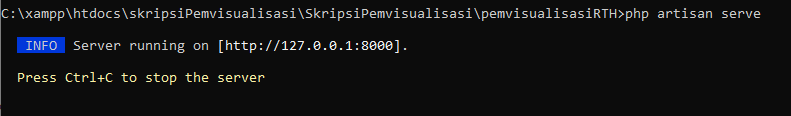
\includegraphics[width=0.5\textwidth]{Gambar/artisan.png}
		\caption{PHP Artisan Laravel}
		\label{fig:artisan}
	\end{figure}
	
	\item \textit{Routing} \\
	\textit{Routing} merupakan suatu proses yang dapat memindahkan tampilan halaman ke halaman lain. Dengan menggunakan \textit{routing}, pengguna dapat menentukan halaman yang ingin dikunjungi. Pengaturan \textit{routing} di laravel terletak pada file \textit{web.php}.
	
	\item \textit{Controller} \\
	\textit{Controller} merupakan suatu proses yang bertujuan untuk mengambil data, menambahkan data, menghapus data, atau mengubah data untuk ditampilkan dalam halaman. Cara membuat \textit{controller} adalah dengan menggunakan \textit{command line} dengan memasukkan "php artisan make controller <<nama\_controller>>". File \textit{controller} nantinya akan otomatis terbuat dan sudah masuk ke folder \textit{controller}.
	
	\item \textit{Blade View} \\
	Blade adalah template \textit{engine} bawaan dari laravel. Blade memiliki kode kode yang lebih mudah untuk menghasilkan laravel. Cara membuat file blade dilakukan secara manual dengan membuat nama\textunderscore file.php.blade di dalam folder views
\end{enumerate}

